\documentclass [11pt,a4paper,oneside,draft]{article}

\usepackage[italian]{babel}
\usepackage[utf8]{inputenc}
\usepackage{indentfirst}
\usepackage{graphicx}
\usepackage{geometry}
\usepackage{verbatim}

% Informations
\title{Implementazione del gioco del blackjack in VHDL}
\author{Emanuele Aina (matr. 129548)}
\date{}

% Margins
\geometry{bindingoffset=0.5cm}

% Caption
\newcommand{\mc}[1]{{\small\ #1}}
\newcommand{\makecaption}[1]{\caption{\mc\ #1}}

% URL
\newcommand{\url}[2]{#1\footnote{#2}}

% References
\newcommand{\refemph}[1]{\emph{#1}}
\newcommand{\imgref}[1]{\refemph{\ref{img:#1}}}
\newcommand{\imgrefx}[1]{\refemph{figura}~\imgref{#1}}

% Images
\newcommand{\im}[3]{
    \begin{figure}[!htb]
        \begin{center}
            \includegraphics{img/#1}
            \makecaption{#2}
            \label{img:#3}
        \end{center}
    \end{figure}
}

% Ignore the argument
\newcommand{\noop}[1]{}

% Foreign words
\newcommand{\foreign}[1]{\emph{#1}}

% Justify even if it has to leave a lot of blank space
\setlength{\emergencystretch}{3em}


\begin{document}

\maketitle

\begin{center}
\small{01GSS - Specifica e simulazione dei sistemi digitali}
\end{center}

\section{Specifiche di progetto}
Si progetti, a livello RT, un circuito che permetta di giocare al gioco del Blackjack.

\subsection{Spiegazione del gioco}
Il gioco si svolge tra due giocatori, di seguito denominati
Giocatore e Banco, con un mazzo di carte da poker. Inizia a giocare il Giocatore,
decidendo se estrarre una carta dal mazzo, oppure passare la mano al Banco. Ad ogni
estrazione, il valore della carta estratta viene sommata al punteggio corrente: lo scopo
è arrivare a totalizzare un punteggio il più vicino possibile a 21, senza mai superarlo.
Se tale valore viene superato durante la mano del Giocatore, il Banco vince
immediatamente. Viceversa, il Banco comincia ad estrarre carte dal mazzo con lo
scopo di realizzare un punteggio almeno pari a quello del Giocatore, senza comunque
superare il limite di 21. Se ciò non accade, vince il Giocatore.

\subsection{Implementazione}
Il circuito possiede quattro ingressi di controllo Reset, NewGame,
Stop ed En di parallelismo pari ad 1 bit e un ingresso di dato I di parallelismo pari a
3 bit, e si deve comportare nel seguente modo:

\begin{itemize}
\item Se Reset = 1, il circuito si porta sempre nello stato iniziale, in cui tutti i led e le
      4 cifre del display a 7 segmenti sono spenti, indipendentemente dal valore
      degli altri segnali.

\item La prima volta che il segnale NewGame assume il valore 1, il sistema si
      prepara a giocare una nuova partita: le due cifre più a destra del display a 7
      segmenti si accendono, riportando il valore del punteggio iniziale (ovvero 00)
      del Giocatore, mentre le due cifre più a sinistra del display e i led sono spenti.

\item Dopo aver iniziato una partita, ogni volta che En assume il valore 1, i segnali
      dell'ingresso di dato I vengono campionati e memorizzati. Essi rappresentano
      il valore, in binario, della carta estratta dal mazzo (si utilizzano carte con valori
      limitati tra 1 e 8, dove il valore 8 è codificato su tre bit come 000). Tale valore
      deve essere visualizzato sui led, ed essere sommato al punteggio corrente.

\item Nel momento in cui il segnale Stop si porta a 1, la mano passa al Banco: le
      due cifre più a sinistra del display a 7 segmenti si accendono e riportano il
      valore iniziale del punteggio del Banco (di nuovo, 00). Analogamente al passo
      precedente, ogni volta che il segnale assume il valore 1, una carta viene
      estratta dal mazzo, il suo valore viene visualizzato sui led e sommato al
      punteggio del Banco.

\item La partita termina quando:
      \begin{itemize}
      \item Il Banco ha totalizzato un punteggio superiore a quello del Giocatore,
            senza eccedere il limite di 21. In questo caso, i punti decimali relativi
            alle due cifre del punteggio del Banco si accendono.

      \item Il Banco ha totalizzato un punteggio superiore al limite di 21: in questo
            caso, si illuminano i punti decimali relativi alle due cifre che riportano il
            punteggio del Giocatore.

      \item Durante la sua mano, il Giocatore ha ottenuto un punteggio superiore a
            21: come nel primo caso, si illuminano i punti decimali delle due cifre
            del punteggio del Banco. Si noti che in questo caso il Banco non gioca
            affatto, quindi i punti decimali si devono accendere, ma le due cifre del
            display a 7 segmenti devono rimanere spente.
      \end{itemize}

\item A questo punto, il sistema si ferma e aspetta che il segnale NewGame si riporti
      a 1, in modo da iniziare una nuova partita.
\end{itemize}

Si implementi il circuito richiesto sulla FPGA in dotazione, utilizzando i bottoni BTN3,
BTN2, BTN1 e BTN0 per i segnali di Reset, NewGame, Stop ed En, e gli switch
SW7, SW6 e SW5 per il segnale di dato I. Il circuito lavori ad una frequenza di clock
pari a 50 kHz.

Si osservi che:
\begin{itemize}
\item Il numero visualizzato sul display deve essere codificato in base 10 (quindi, se
      il suo valore è 19 e viene incrementato, il nuovo valore da visualizzare è
      effettivamente 20, non 1A).

\item I led da illuminare ogni volta che una carta viene estratta sono in numero pari
      al valore della carta, e partono sempre da LD0. Per esempio, se la carta
      estratta ha un valori pari a 3, si devono illuminare i led LD0, LD1 e LD2.
\end{itemize}


\section{Implementazione}
\subsection{Metodologia}
Il progetto è stato implementato esclusivamente mediante descrizioni VHDL, sia a
livello comportamentale che a livello strutturale.

Lo sviluppo è avvenuto in ambiente Linux (Debian etch) utilizzando GHDL 0.25 per le
simulazioni e, successivamente, in ambiente Windows con Xilinx 6.1i per la
programmazione su FPGA.

Per ogni componente sviluppato è stato inoltre realizzato un testbench in VHDL 
puro, in modo da renderne possibile la verifica in modo automatico (make run). %FIXME

\subsection{Board}
Il componente ``board'' rappresenta l'entità di più alto livello e costituisce
la parte del progetto che verrà programmata sulla FPGA.

\verbatiminput{board/board.vhdl}

La descrizione è strutturale e provvede a istanziare i componenti ``blackjack''
e ``display'' connettendoli tra loro e a impiegare ``clock\_divider'' per 
convertire il clock della scheda a frequenze inferiori per la logica di 
gioco e per la logica di gestione del display. I segnali di input vengono 
inoltre filtrati usando dei generatori di impulsi al fine di evitare 
campionamenti multipli di una singola pressione.

Il componente è dotato del seguente testbench per la verifica automatica.

\verbatiminput{board/tb_board.vhdl}

Oltre all'unità da verificare, viene anche istanziato un simulatore per il
sistema di gestione dei display a sette segmenti disponibili sulla FPGA,
controllando il funzionamento della logica di codifica e multiplexing.

Il clock viene generato con un periodo di 1ns fino a che non esistano più
eventi per la simulazione. A tal punto anche il clock viene fermato in 
modo da segnalare al simulatore la fine del test.

Il processo ``count'' si limita a conteggiare il numero di colpi di clock
in modo che il processo ``test'' possa impostare i vettori di test con 
la cadenza specificata. Questo processo, infatti, si occupa di leggere
i vettori di input e gli output attesi da un file e applicarli all'unità
testata. Nel caso specifico, dovendo simulare l'input dell'utente, la
frequenza con cui gli input vengono applicati è nell'ordine dei 
millisecondi anziché dei nanosecondi usati dal clock di simulazione.

\verbatiminput{board/tb_board.test}

Su ogni riga è specificato l'istante corrispondente, gli input e gli
output.

\subsection{Blackjack}
Il componente ``blackjack'' contiene l'intera logica di gioco descritta
nelle specifiche, utilizzando al suo interno i componenti
``game\_logic'', il quale implementa le regole di vittoria/perdita,
``fsm'', che determina gli stati di gioco, ``bcd\_encoder'' per
convertire i punteggi in Binary Coded Decimal, nonché ``reg'' e ``rca'',
rispettivamente un registro PIPO e un Ripple Carry Adder.


\verbatiminput{blackjack/blackjack.vhdl}

Anche qui la descrizione è strutturale e si occupa di istanziare e 
interconnettere i componenti presenti. In particolare i due registri
sono usati per memorizzare il punteggio del Giocatore e del Mazziere:
a ciascuno è connesso un sommatore il quale somma il punteggio con il
valore in input ed è usato per calcolare il punteggio futuro.
``game\_logic'' determina se uno tra Giocatore o Mazziere ha vinto o
ha sballato al fine di segnalarlo alla macchina a stati, la quale
reagirà opportunamente. Entrambi i punteggi vengono poi convertiti in
BCD a due cifre.

\verbatiminput{blackjack/tb_blackjack.test}

I vettori di test simulano una serie di partite controllando il 
comportamente del sistema in alcune situazioni plausibili.
In questo caso a ogni riga corrisponde un colpo di clock, per cui
è necessario consentire alla macchina a stati il tempo necessario
a compiere le proprie funzioni, essendo l'unico componente a non
reagire nell'arco di un periodo di clock. Il codice VHDL del 
testbench è stato omesso essendo analogo a quanto visto nel caso del
componente ``board''.

\subsection{Fsm}

La macchina a stati si occupa di gestire le differenti fasi del gioco,
nonché di controllare l'acquisizione e la verifica dei valori in input
e di prendere le opportune decisioni. Questo è l'unico componente
realizzato il cui modo di operare richiede più colpi di clock: questa
è una scelta voluta, in modo da concentrare la logica per la gestione
delle tempistiche e degli stati in un singolo componente.

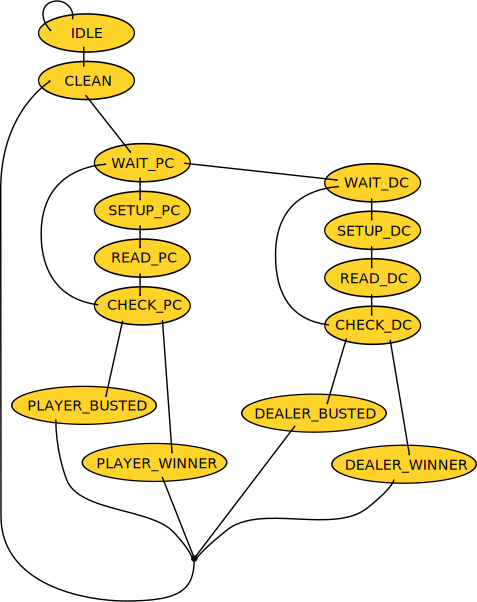
\includegraphics{fsm}

Lo stato iniziale è lo stato di ``IDLE'', nel quale la macchina resta
in attesa di eventi. Da qui ``CLEAN'' imposta le condizioni iniziali
del gioco, in modo da permettere il funzionamento degli stati successivi.
Tra questi, quelli i cui nomi
terminano con ``PC'' sono relativi al turno del Giocatore, mentre 
quelli con ``DC'' spettano al Mazziere. Questi rappresentano le fasi
di attesa, acquisizione e controllo dei valori in input, mentre quelli
che terminano con ``BUSTED'' o ``WINNER'' indicano le condizioni 
terminali del gioco.

\verbatiminput{fsm/fsm.vhdl}

La macchina a stati è stata costruita con tre processi: uno molto 
semplice per propagare lo stato futuro, uno per determinare quale
questo sia in funzione degli input e uno per determinare gli output
in funzione delllo stato corrente.

\verbatiminput{fsm/tb_fsm.test}

\subsection{game\_logic}

La logica che determina la vittoria o la sconfitta dei giocatori è
contenuta nel componente combinatorio ``game\_logic'', il quale
si occupa di controllare i punteggi nel caso questi superino 21 o
che si sia verificata una delle condizioni di vittoria.

\verbatiminput{game_logic/game_logic.vhdl}

La descrizione è comportamentale e prevede un processo per ciascun
output, utilizzando il tipo ``unsigned'' per effettuare i confronti
tra i punteggi.

\verbatiminput{game_logic/tb_game_logic.vhdl}

Essendo il componente combinatorio, il testbench risulta essere
leggermente più semplice rispetto a quelli impiegati per i componenti
precedenti, seppur rimanendo molto simile.

\verbatiminput{game_logic/tb_game_logic.test}

Il test si limita a sottoporre al circuito alcune situazioni di 
gioco senza un ordine particolare, valutando l'esito di ciascuna.

\subsection{reg}

L'entità ``reg'' descrive un semplice registro PIPO sincrono dotato di 
segnale di abilitazione (``EN'') oltre agli ingressi (``A'') e alle
uscite (``O''). Il parametro ``N'' permette di impostare la dimensione
in bit del registro.

\verbatiminput{reg/reg.vhdl}

La stessa entità è stata implementata sia con una descrizione
comportamentale che con una strutturale. La prima contiene
il costrutto condizionale comunemente usato per implementare
circuiti sincroni con segnale di reset asincrono e un semplice
assegnamento, mentre la seconda istanzia in un ciclo un vettore
di flip-flop di tipo D a cui connette ingressi e uscire.

\verbatiminput{reg/tb_reg.test}

Il test viene eseguito con un registro a tre bit verificandone
il comportamento.

\end{document}
